%\documentclass[submission]{eptcs}
\documentclass[submission]{eptcs}
\providecommand{\event}{TTC 2015}

\usepackage[usenames,dvipsnames,table]{xcolor}
\usepackage[T1]{fontenc}
\usepackage{geometry}
\usepackage{paralist}
\usepackage{graphicx}
\usepackage[cache]{minted}
\usepackage{url}
\usepackage[utf8]{inputenc}
\usepackage{paralist}
\usepackage{amstext}
\usepackage{amsfonts}
\usepackage{xspace}
\usepackage{todonotes}
\usepackage{hyperref}

\usepackage[skip=0pt]{caption}
\usepackage{setspace}
\setstretch{0.96}

\hypersetup{
  colorlinks, 
  breaklinks, 
  bookmarksnumbered=true,
  pdftitle={Solving the TTC'15 Train Benchmark Case Study with SIGMA},
  pdfauthor={Filip Křikava}, 
  linkcolor=Blue, 
  citecolor=BrickRed, 
  filecolor=Blue, 
  urlcolor=Blue
  }

\renewcommand{\ttdefault}{pcr}

\newcommand{\SIGMA}{\textsc{Sigma}\xspace}
\newcommand{\FIXML}{FIXML\xspace}
\newcommand{\TTC}{TTC'15\xspace}
\newcommand{\Ie}{\emph{i.e.}\xspace}
\newcommand{\Eg}{\emph{e.g.}\xspace}
\newcommand{\Etal}{\emph{et al.}\xspace}
\newcommand{\Cf}{\emph{cf.}\xspace}

\newcommand{\Todo}[1]{\todo[inline]{#1}}
\renewcommand{\Todo}[1]{}

\newminted{scala}{fontsize=\fontsize{8}{8},linenos,numbersep=5pt,frame=lines,framesep=2mm}
\newminted{bash}{fontsize=\fontsize{8}{8},linenos,numbersep=5pt,frame=lines,framesep=2mm}

\newcommand{\Scala}[1]{\mintinline{scala}{#1}}

\title{Solving the \TTC Train Benchmark Case Study with SIGMA}

\author{
  Filip Křikava
  \institute{University Lille 1 - LIFL, France}
  \institute{INRIA Lille, Nord Europe}
  \email{\href{mailto:filip.krikava@inria.fr}{filip.krikava@inria.fr}}
% \and
%   Philippe Collet
%   \institute{Université Nice - Sophia Antipolis, France}
%   \institute{CNRS, I3S, UMR 7271}
%   \email{\quad \href{mailto:philippe.collet@unice.fr}{philippe.collet@unice.fr}}
}

\def\titlerunning{Solving the \TTC Train Benchmark Case Study with SIGMA}
\def\authorrunning{F. Křikava}

\begin{document}
\maketitle

\begin{abstract}
In this paper we describe a solution for the \emph{Transformation Tool Contest 2015} (\TTC) Train Benchmark case study using \SIGMA, a family of Scala internal \emph{Domain-Specific Languages} (DSLs) that provides an expressive and efficient API for model consistency checking and model transformations.
We solve both the core and the extension tasks.
\end{abstract}

%!TEX root = ttc15-train-benchmark-sigma.tex

% \enlargethispage{10mm}

\section{Introduction}
\label{sec:Introduction}

%% Overview
In this paper we describe our solution for the \TTC Train Benchmark case study~\cite{Szarnyas2015} using the \SIGMA~\cite{Krikava2014}.
%% Scala
\SIGMA is a family of Scala\footnote{\url{http://scala-lang.org}} internal DSLs for model manipulation tasks such as model validation, model to model (M2M), and model to text (M2T) transformations.
Scala is a statically typed production-ready \emph{General-Purpose Language} (GPL) that supports both object-oriented and functional styles of programming.
It uses type inference to combine static type safety with a \emph{``look and feel''} close to dynamically typed languages.
Furthermore, it is supported by the major integrated development environments bringing EMF modeling to other IDEs than traditionally Eclipse (the solution was developed in IntelliJ IDEA\footnote{\url{https://www.jetbrains.com/idea/}}).

%% SIGMA
\SIGMA DSLs are embedded in Scala as a library allowing one to manipulate models using high-level constructs similar to the ones found in the external model manipulation DSLs.
The intent is to provide an approach that developers can use to implement many of the practical model manipulations within a familiar environment, with a reduced learning overhead as well as improved usability and performance.
The solution is based on the \emph{Eclipse Modeling Framework} (EMF)~\cite{EMF}, which is a popular meta-modeling framework widely used in both academia and industry, and which is directly supported by \SIGMA.

%% Organization
The complete source code is available on Github\footnote{\url{https://github.com/fikovnik/trainbenchmark-ttc}} in the fork of the original case study repository.
In the Appendix~\ref{sec:Install} we provide a steps how to install it locally.
%!TEX root = ttc15-train-benchmark-sigma.tex

% \enlargethispage{20mm}

\section{Solution Description}
\label{sec:SolutionDescription}

Essentially, the solution for this transformation case study consist of queries that check for violations of a number of constrains and repair transformations that fixes them.
\SIGMA provides a dedicated model consistency checking DSL with the ability to provide quick fixes repairing invariant validations.
However, given the structure of the case study source, we realize the solution in the way it can be easily compared to the reference implementations in both Java and EMF-IncQuery.
Another reason is that it shows that \SIGMA can be easily integrated in existing modeling projects and other high-level abstractions can be easily developed.
We therefore only rely on the \SIGMA common infrastructure which provides a set of basic operations for model navigation (\Ie projecting information from models) and modification (\Ie changing model properties or elements).

The description of the solution is split in two parts:
\begin{inparaenum}[(1)]
  \item the core part that describes the queries and repair transformations,
  \item the integration part gives an overview how it has been integrated in the case study source code.
\end{inparaenum}

The solution has been implemented in a separate module \texttt{hu.bme.mit.trainbenchmark. ttc.benchmark.sigma} in a fork of the original code based provided by the case study.

\subsection{Queries and Repair Transformations}

Essentially, we have created a small internal DSL that builds on \SIGMA that allows us to solve the given benchmark cases in an expressive and compact way---\Ie to express the model queries and repair transformations.

The top-level constructs in the DSL is a \emph{constraint}.
A constraint is composed of a model \emph{query} that finds all model instances violating a certain model restriction and a \emph{repair} transformation correcting the failed instances.
Concretely, a query is a function that given a model element---\Ie a context of the constraint in the classical model consistency checking---returns a set of \emph{matches}.
A match can be either a singe instance or a tuple of instances of model elements that are related to the violations.

\subsection{Constraint DSL}

A typical way of creating an internal DSL in Scala is by designing a library that allows one to write fragments of code with domain-specific syntax.
These fragments are woven within Scala own syntax so that it appears different.

One way to represent the above concepts is using a Scala case class:
%
\begin{scalacode}
case class Constraint[A <: EObject, B <: AnyRef](
  query: (A) => Iterable[B],
  repair: (B) => Unit
)
\end{scalacode}
%
This defines a case class with a field for both query and repair.
A case class in Scala is like a regular class which some additional properties out which, in our case, the important one is that it can be instantiated without the \texttt{new} keyword and thus limiting the language noise.
The two type parameters \texttt{A, B} specify the model context for the query and the types of matches the query produces.
The input type is further constrained to be a subtype of an \texttt{EObject}.

Given this case class we can write a constraint using:
%
\begin{scalacode}
Constraint[A, (B, C)](
  query = ...
  repair = ...
)
\end{scalacode}
%
The query and repair are defined as functions \texttt{A} $\rightarrow$ \texttt{Iterable[B]} and \texttt{B} $\rightarrow$ \texttt{Unit} where \texttt{Unit} is like \texttt{void} in Java.

In some cases the match returned by the query is of the same type as the query context.
The query can be therefore simplified to a boolean expression selecting instances on which it evaluates to true.
For these type of queries we provide a dedicated constructs called \texttt{BooleanConstraint}:
%
\begin{scalacode}
case class BooleanConstraint[A <: EObject : ClassTag](
  query: (A) => Boolean, 
  repair: (A) => Unit
)
\end{scalacode}

For example, the first query, \emph{PosLength}, which finds all the segments with negative length can be written as:
%
\begin{scalacode}
BooleanConstraint[Segment](
  query = segment => segment.length < 0,
  repair = segment => segment.length += -segment.length + 1
)
\end{scalacode}
%
In Scala, \texttt{name => ...} is a function literal of one parameter function.
We do not have to specify the types of the parameter nor the result as they will be inferred by the Scala compiler.

Next to constraint, we define a validator that allows one to check and consequently repair the incorrect model instances:
%
\begin{scalacode}
abstract class Validator[A <: EObject, B <: AnyRef] {
  def check(container: EObject): Iterator[B]
  def repair(matches: Iterator[B]): Unit
}
\end{scalacode}
%
It is defined as an abstract class with two methods that correspond to the two operations we want to do---\Ie check and repair.
Finally, we provide an implementation for the two types of queries that we have:
%
\begin{scalacode}
case class ConstraintValidator[A <: EObject, B <: AnyRef](constraint: Constraint[A, B]) 
  extends Validator[A, B] {
  
  override def check(container: EObject) =
    container.eAllContents collect { case x: A => x } flatMap constraint.query

  override def repair(matches: Iterator[B]) = 
    matches foreach constraint.repair
}
\end{scalacode}
%
The implementation is straight forward.
For all elements contained in a \texttt{container}, we first collect all instances of the required context type and then query them using the query function provided by the given constraint.
The repair simply executes the constraint repair function on the matching element.

The DSL is implemented in a Scala file \texttt{hu/bme/mit/trainbenchmark/ttc/benchmark/sigma/ConstraintDSL.scala}.

\subsubsection{Constraints}

In the following we describe the individual constraints that were part of the case study (case study tasks) except the \emph{PosLength} that has already been shown above.

\begin{itemize}[---]
  \item \emph{SwitchSensor}
  %
  \begin{scalacode}
  BooleanConstraint[Switch](
    query = switch => switch.sensor.isEmpty,
    repair = switch => switch.sensor = Sensor()
  )
  \end{scalacode}
  %
  The \texttt{isEmpty} is a method that is defined on an \texttt{Option} type (coming from the standard Scala library) representing a type which may or may not have a value.
  Since in the model, the \emph{sensor} reference of the \texttt{Switch} class is defined as optional (with cardinality \texttt{0..1}), in \SIGMA we represent the reference using the \texttt{Option} class.
  Not only makes this the cardinality expressed in the type definition, but it also prevents some of the \texttt{NullPointerException}s caused by traversing unset references.
  Technically, this is realized by implicit conversions (\Cf Krikava~\Etal \cite{Krikava2014}).

  \item \emph{SwitchSet}
  %
  \begin{scalacode}
  Constraint[SwitchPosition, (Semaphore, Route, SwitchPosition, Switch)](
    query = swP => {
      for {
        semaphore <- Option(swP.route.entry) if semaphore.signal == Signal.GO
        sw = swP.switch if sw.currentPosition != swP.position
      } yield (semaphore, swP.route, swP, sw)
    },

    repair = {
      case (_, _, swP, sw) => sw.currentPosition = swP.position
    }
  )
  \end{scalacode}
  %
  This is a more complex constraint that matches a tuple of model elements.
  It is using a \emph{for comprehension}, a lightweight notation for expressing sequence comprehensions.
  From the Scala documentation\footnote{\url{http://docs.scala-lang.org/tutorials/tour/sequence-comprehensions.html}}:
  Comprehensions have the form \Scala{for (enumerators) yield e}, where enumerators refers to a semicolon- or new line-separated list of enumerators.
  An \emph{enumerator} is either a generator which introduces new variables, or it is a filter.
  A comprehension evaluates the body \emph{e} for each binding generated by the enumerators and returns a sequence of these values.
  
  In this concrete example, the generator is the optional value of the \texttt{Route.entry} reference.
  It either generates a single value in the case the actual instance contains one or it does not produce anything.
  Because, there is a mistake in the model (the \texttt{Route.entry} should have the cardinality set to \texttt{0..1} instead of \texttt{1}), we need to explicitly convert the reference to an \texttt{Option}.

  The repair function is defined using a pattern matching construct allowing us to concisely assign variables from the matching tuple.

  \item \emph{RouteSensor}
  %
  \begin{scalacode}
  Constraint[Route, (Route, Sensor, SwitchPosition, Switch)](
    query = route => {
      for {
        swP <- route.follows
        sw = swP.switch
        sensor <- sw.sensor if !(route.definedBy contains sensor)
      } yield (route, sensor, swP, sw)
    },

    repair = {
      case (route, sensor, _, _) => route.definedBy += sensor
    }
  )
  \end{scalacode}
  %
  The implementation is similar to the the previous case.
  It is also based on a for comprehension and closely follows the description of the query.

  \item \emph{SemaphoreNeighbor}
  %
  \begin{scalacode}
  Constraint[Route, (Semaphore, Route, Route, Sensor, Sensor, TrackElement, TrackElement)](
    query = route1 => {
      for {
        sensor1 <- route1.definedBy if route1.exit != null
        te1 <- sensor1.elements
        te2 <- te1.connectsTo
        sensor2 <- te2.sensor
        route2 <- sensor2.sContainer[Route] if route1 != route2
        semaphore = route1.exit if semaphore != route2.entry
      } yield (semaphore, route1, route2, sensor1, sensor2, te1, te2)
    },

    repair = {
      case (semaphore, _, route2, _, _, _, _) => route2.entry = semaphore
    }
  )
  \end{scalacode}
  %
  Again based on the for comprehension.
  Additionally, we provide a shortcut using the \texttt{route1.exit != null} so immediately skip the route instances that do not have an exit semaphore set. 

\end{itemize}

The complete solution is implemented in a Scala object\footnote{A Scala object defines a single instance of a class.} \texttt{hu.bme.mit.trainbenchmark.ttc. benchmark.sigma.Solution}.


\subsection{Integration}

The integration consists in making our solution work within the provided benchmark framework.
For this we simply follow what has been provided for the reference implementation in Java.
The following files were created:

\begin{itemize}[---]
  \item \texttt{SigmaBenchmarkMain.scala} contains the main application running the benchmark.
  \item \texttt{SigmaBenchmarkLogic.scala} contains the logic selecting which benchmark shall be run.
  \item \texttt{SigmaBenchmarkCase.scala} contains the adaptors bridging the framework with our constraint language. 
  This files also defines \texttt{SigmaBenchmarkComparator} that is used to compare the matches as required by the case study.
  It is a general comparator that either compares single instances (results from boolean constraints violations) or tuples (regular constraints violations).
\end{itemize}
%!TEX root = ttc15-train-benchmark-sigma.tex

% \vspace*{-3mm}
% \enlargethispage{7mm}

\section{Evaluation}
\label{sec:Evaluation}

In this section we provide an evaluation of our solution following the categories given by the case study.

\subsection{Correctness and Completeness of Model Queries and Transformations}

We developed a solution for all of the tasks required by the case study and the solution passes the provided tests.

\subsection{Conciseness}

The solution itself consists of 52 lines of Scala code the internal DSL developed for this case study.
The DSL itself has been implemented using 20 lines of Scala code using \SIGMA.
The integration part consists of three files with the total of 65 lines.
All measures are source lines only excluding comments and new lines.
Given these measures, we believe that the code is quite concise.

\subsection{Readability}

Next to being concise, the solution is also quite expressive.
This means that the given problem (queries and repair transformations) naturally maps into the implementation.
The higher-level abstraction provided by both \SIGMA and the internal DSLs helps to facilitate it making a significant improvement over the Java reference implementation.
% It is important to note that we could have provided even a more flexible syntax, but that would obscure the implementation of the DSL (the type definition) and make the possible error messages more cryptic.
%
Next to being concise and expressive, the code is also type-safe as Scala is statically typed language.
A notable consequence is that it is very easy to use the DSL with an IDE like Eclipse or IntelliJ that provides a robust code completing functionalities, outline views and other features increasing one's productivity.

In summary, while readability is a subjective matter and largely depends on the background and experience of users, we believe that \SIGMA scores well.
Thanks to the syntax of Scala which is close to one of Java/C++ and hence shall be familiar to many developers.
The expressiveness of the first-order logic collection operation should be familiar to anyone knowing OCL or any other function language.


\subsection{Performance on Large Models}

The tests have been performed on an 2.3 GHz Intel Core i7 machine with 16 GB of RAM being dedicated to the JVM process.
We ran our solution together with the reference implementation in Java.
We used the model instances from size 1 to 8192 and set 8GB memory to be dedicated to the JVM.
The corresponding results are shown in the figures~\ref{fig:SigmaFixedValidationBatch} and~\ref{fig:SigmaFixedReValidationBatch}.
We compare them to the Java solution which is shown in the figures~\ref{fig:JavaFixedValidationBatch} and~\ref{fig:JavaFixedReValidationBatch}.
We get a similar performance which has been expected due to the fact that Scala compiles directly to Java bytecode and we use the same underlying libraries for accessing EMF models.
This shows that we can leverage from concise and expressive queries without sacrificing performance.

It is important to note that we do not developed any extra functionality for these benchmarks---\Ie no caching or incremental validations.
On the other hand, functional approach we have selected makes it perfect for further parallelization.
Moreover, for even larger models we could easily port the solution into big data analysis platforms such as Hadoop\footnote{\url{https://hadoop.apache.org/}}.
This would be rather difficult given the imperative Java implementation.

\begin{figure}[h!tb]
  \centering
  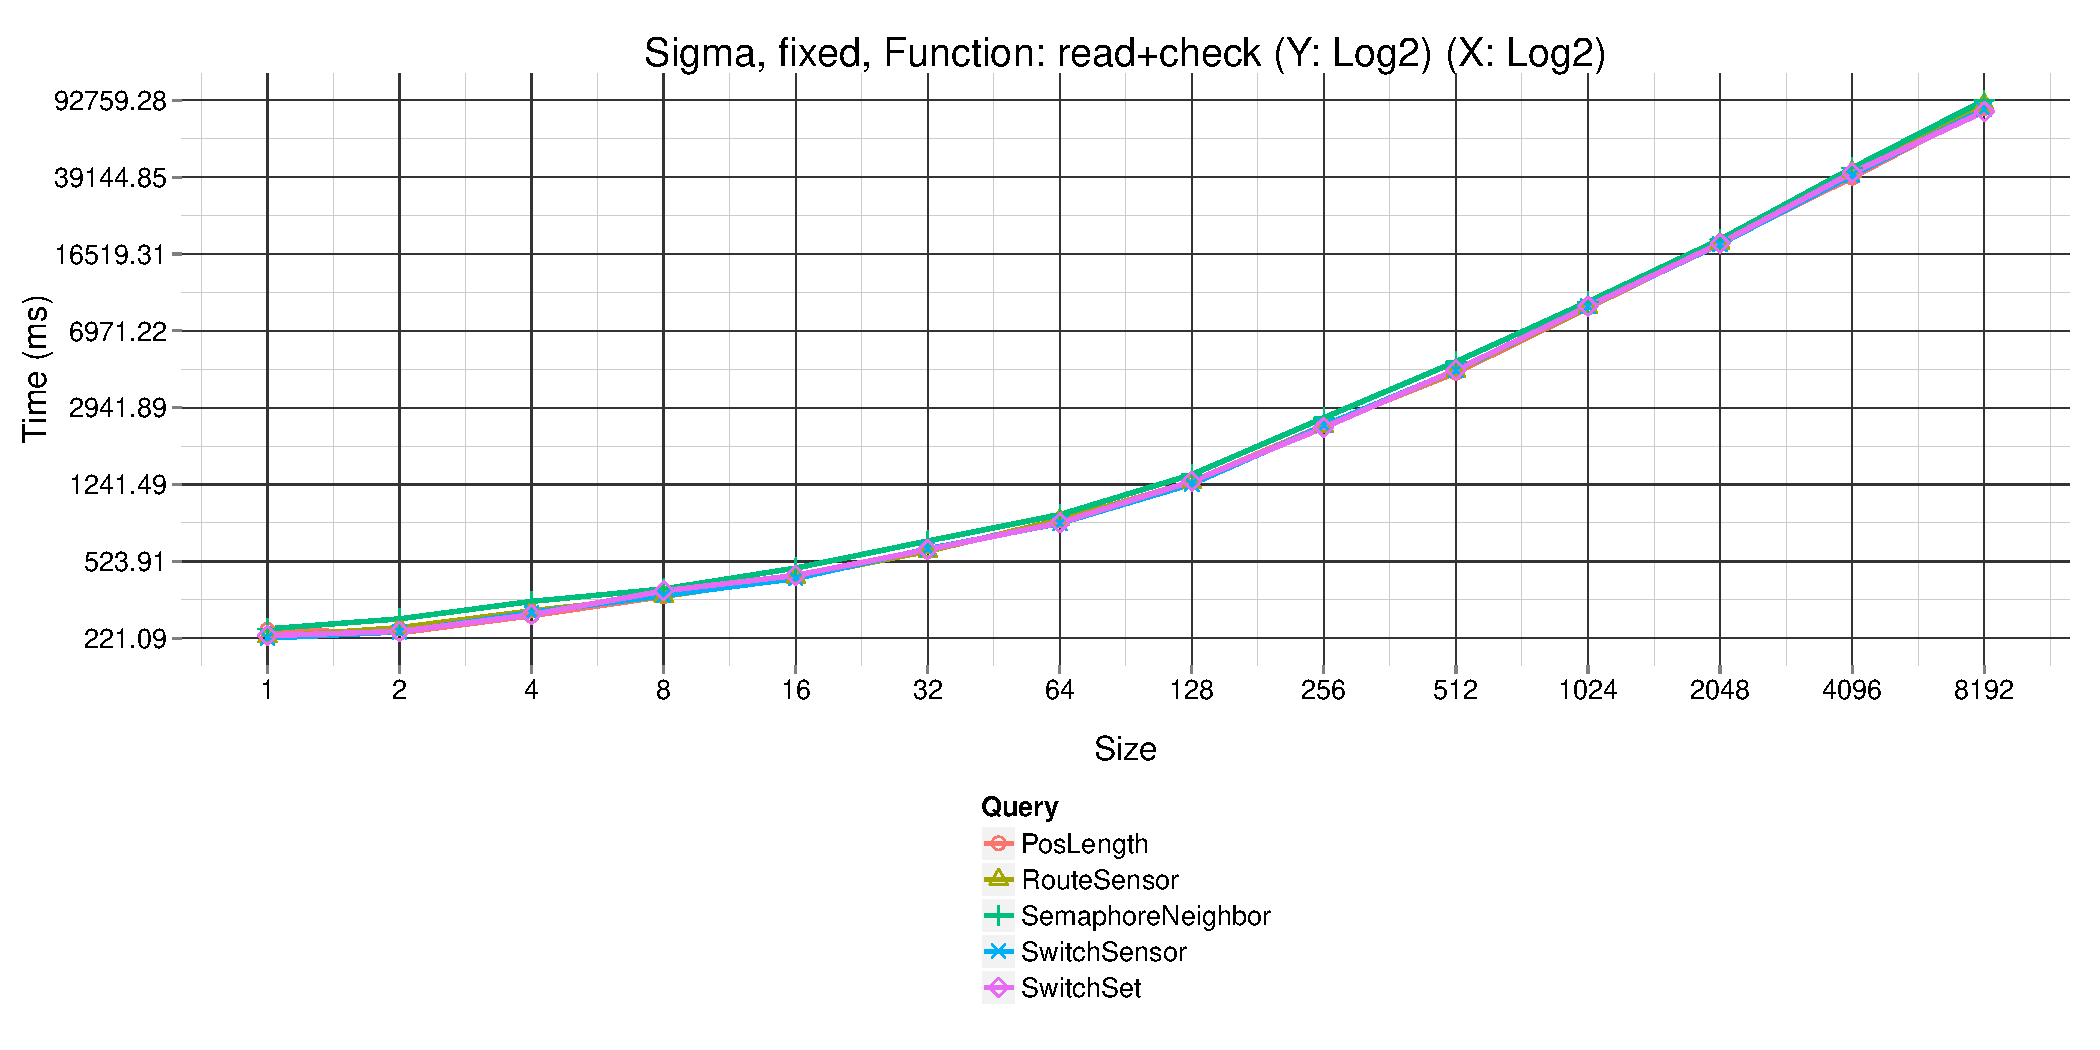
\includegraphics[width=\textwidth]{figures/fixed-Sigma-GroupBy-Query-time-batch-validation.pdf}
  \caption{\SIGMA fixed validation batch}
  \label{fig:SigmaFixedValidationBatch}
\end{figure}

\begin{figure}[h!tb]
  \centering
  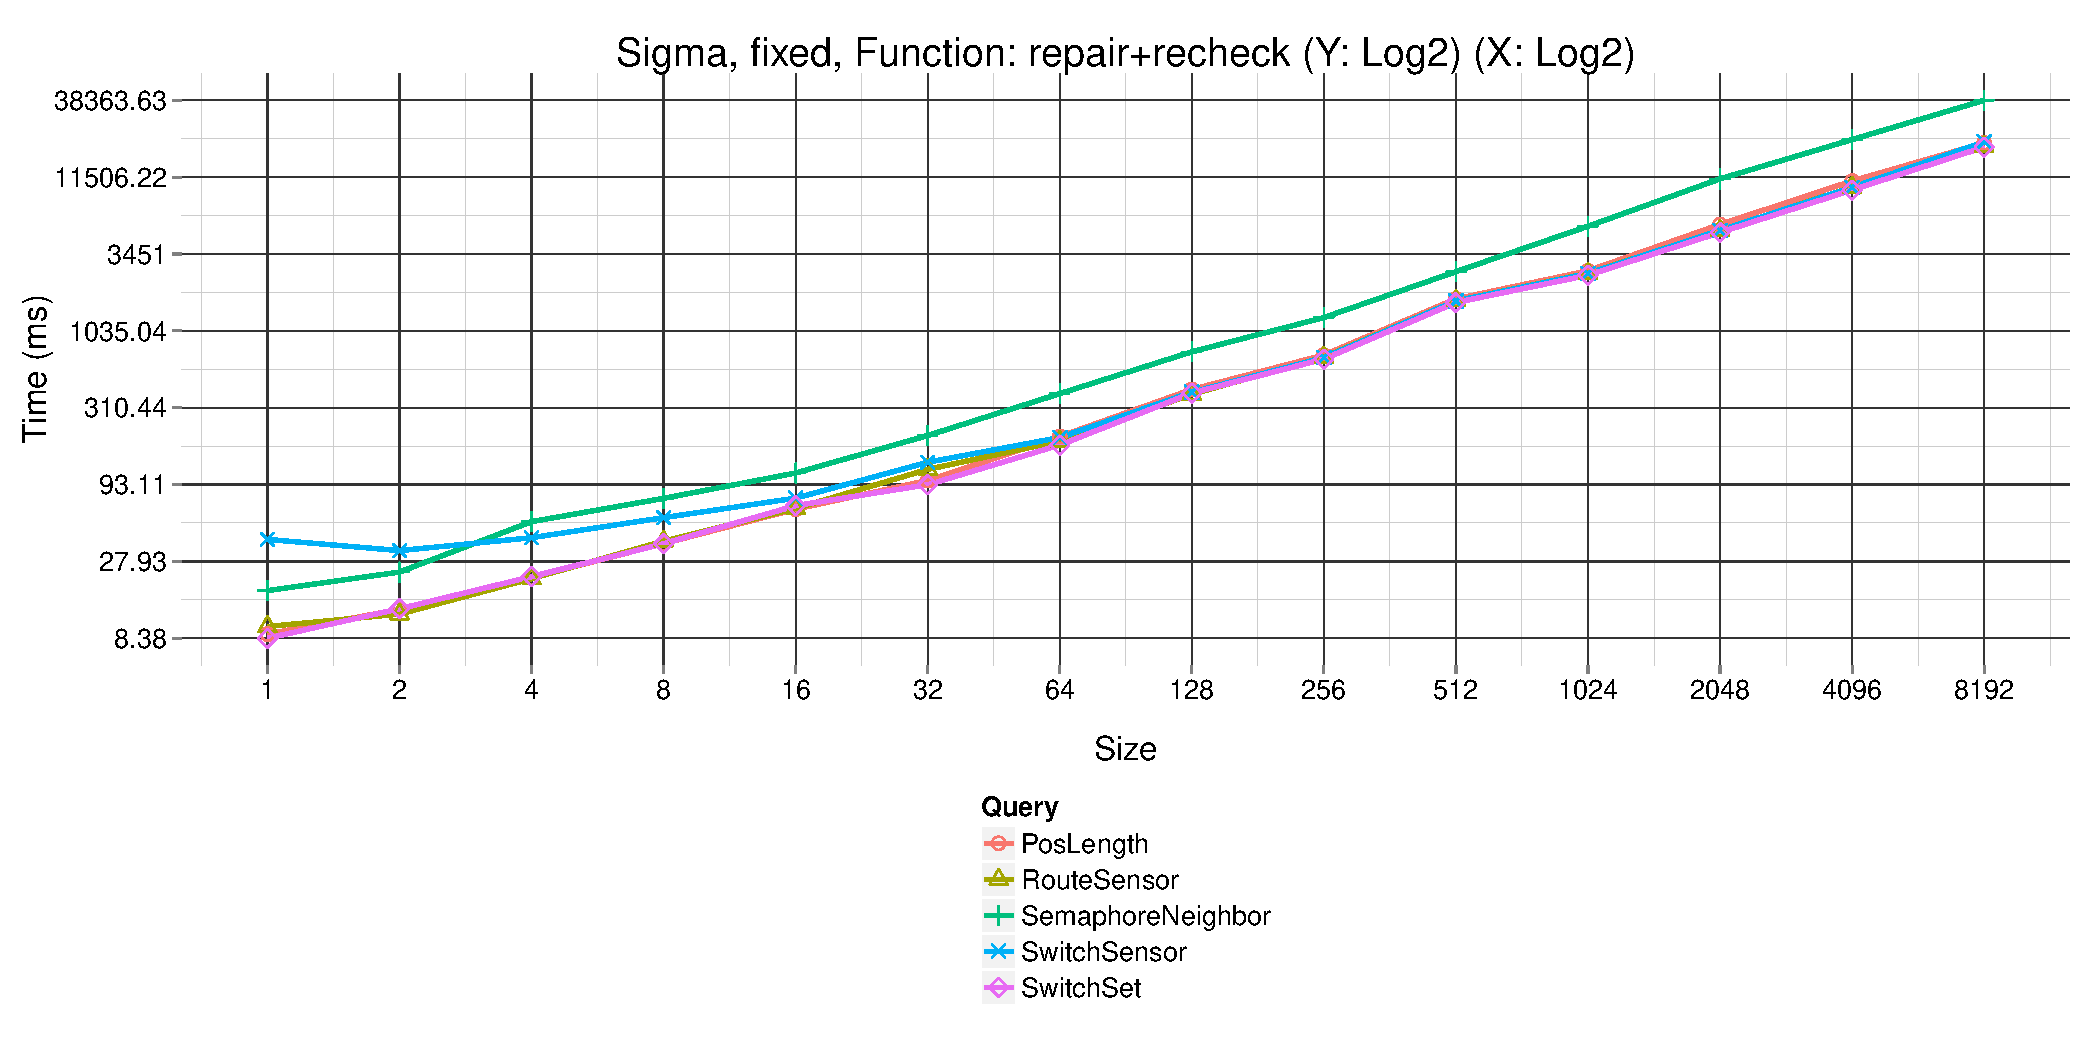
\includegraphics[width=\textwidth]{figures/fixed-Sigma-GroupBy-Query-time-revalidation.pdf}
  \caption{\SIGMA fixed revalidation}
  \label{fig:SigmaFixedReValidationBatch}
\end{figure}

\begin{figure}[h!tb]
  \centering
  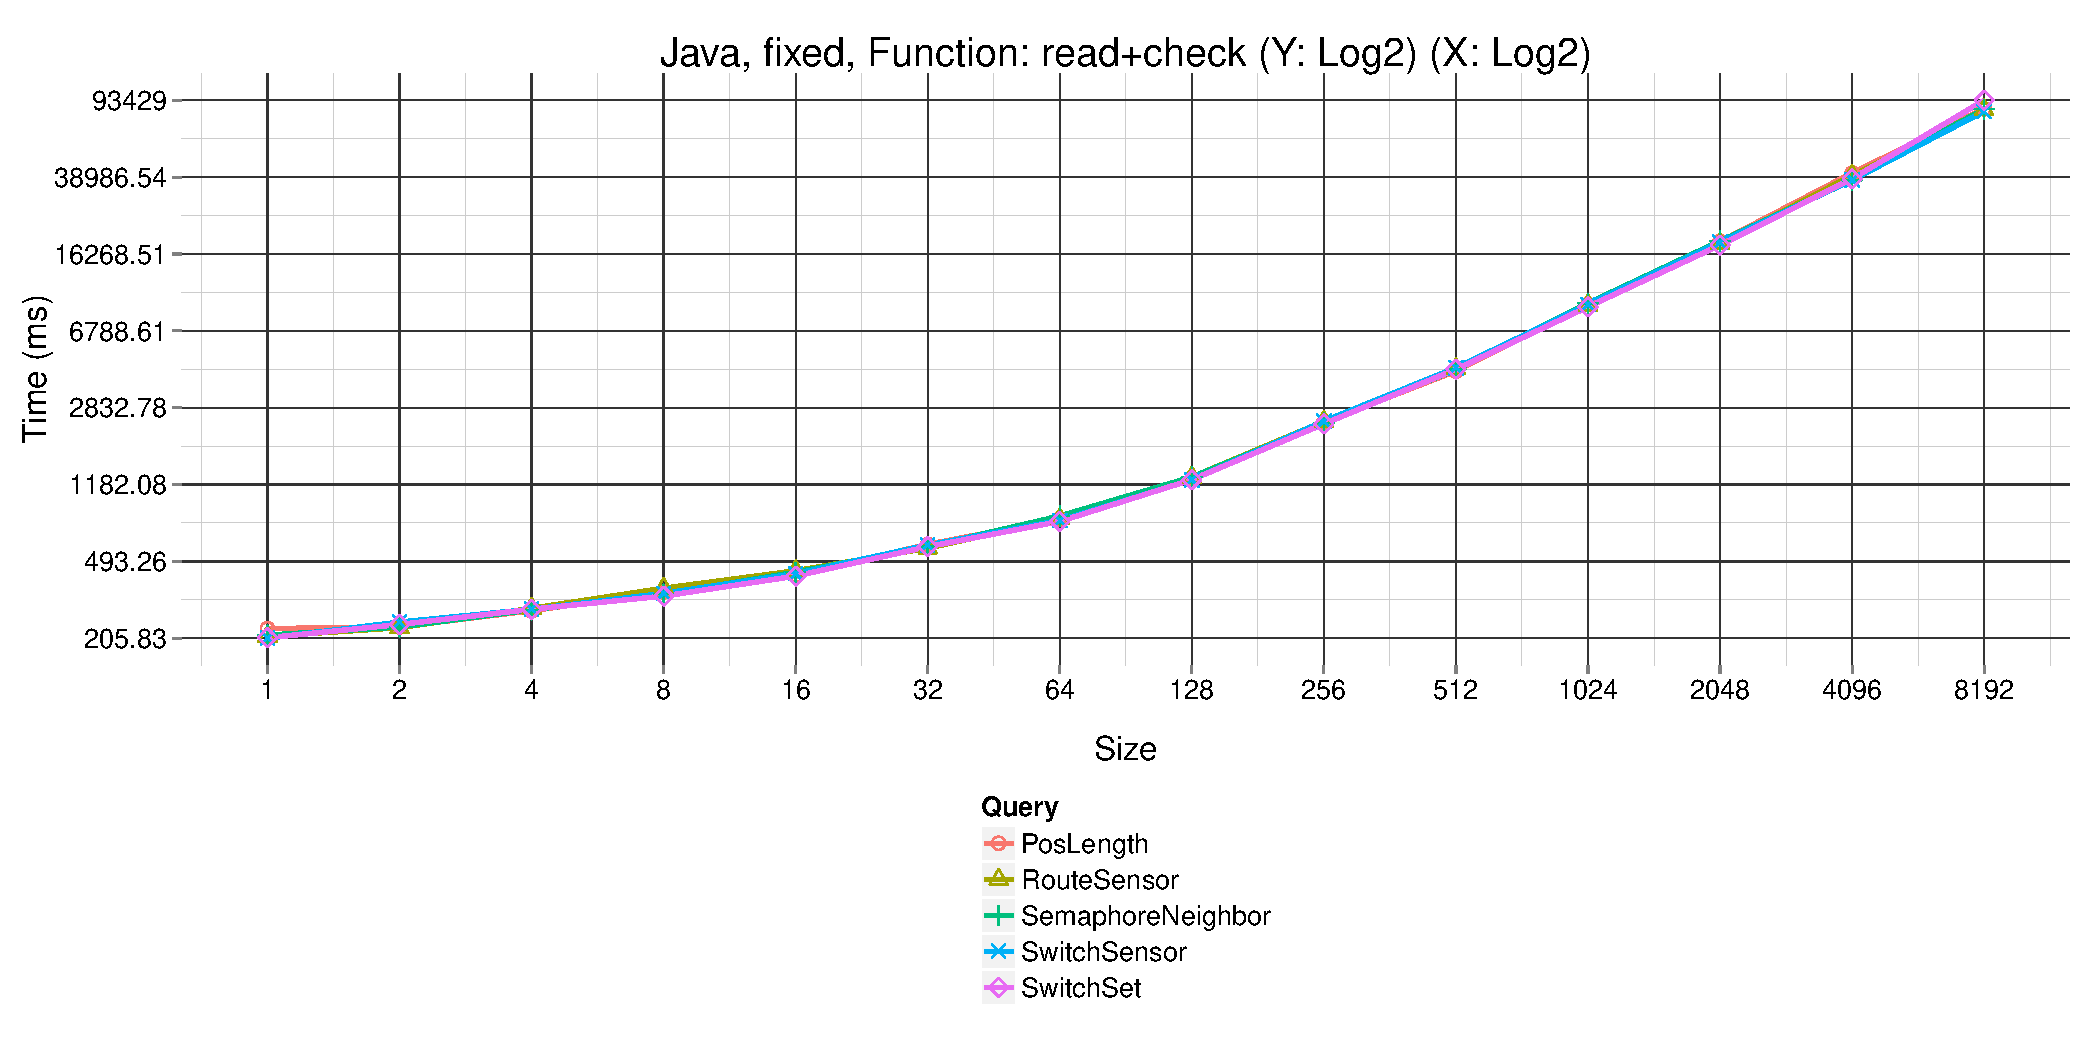
\includegraphics[width=\textwidth]{figures/fixed-Java-GroupBy-Query-time-batch-validation.pdf}
  \caption{Java fixed validation batch}
  \label{fig:JavaFixedValidationBatch}
\end{figure}

\begin{figure}[h!tb]
  \centering
  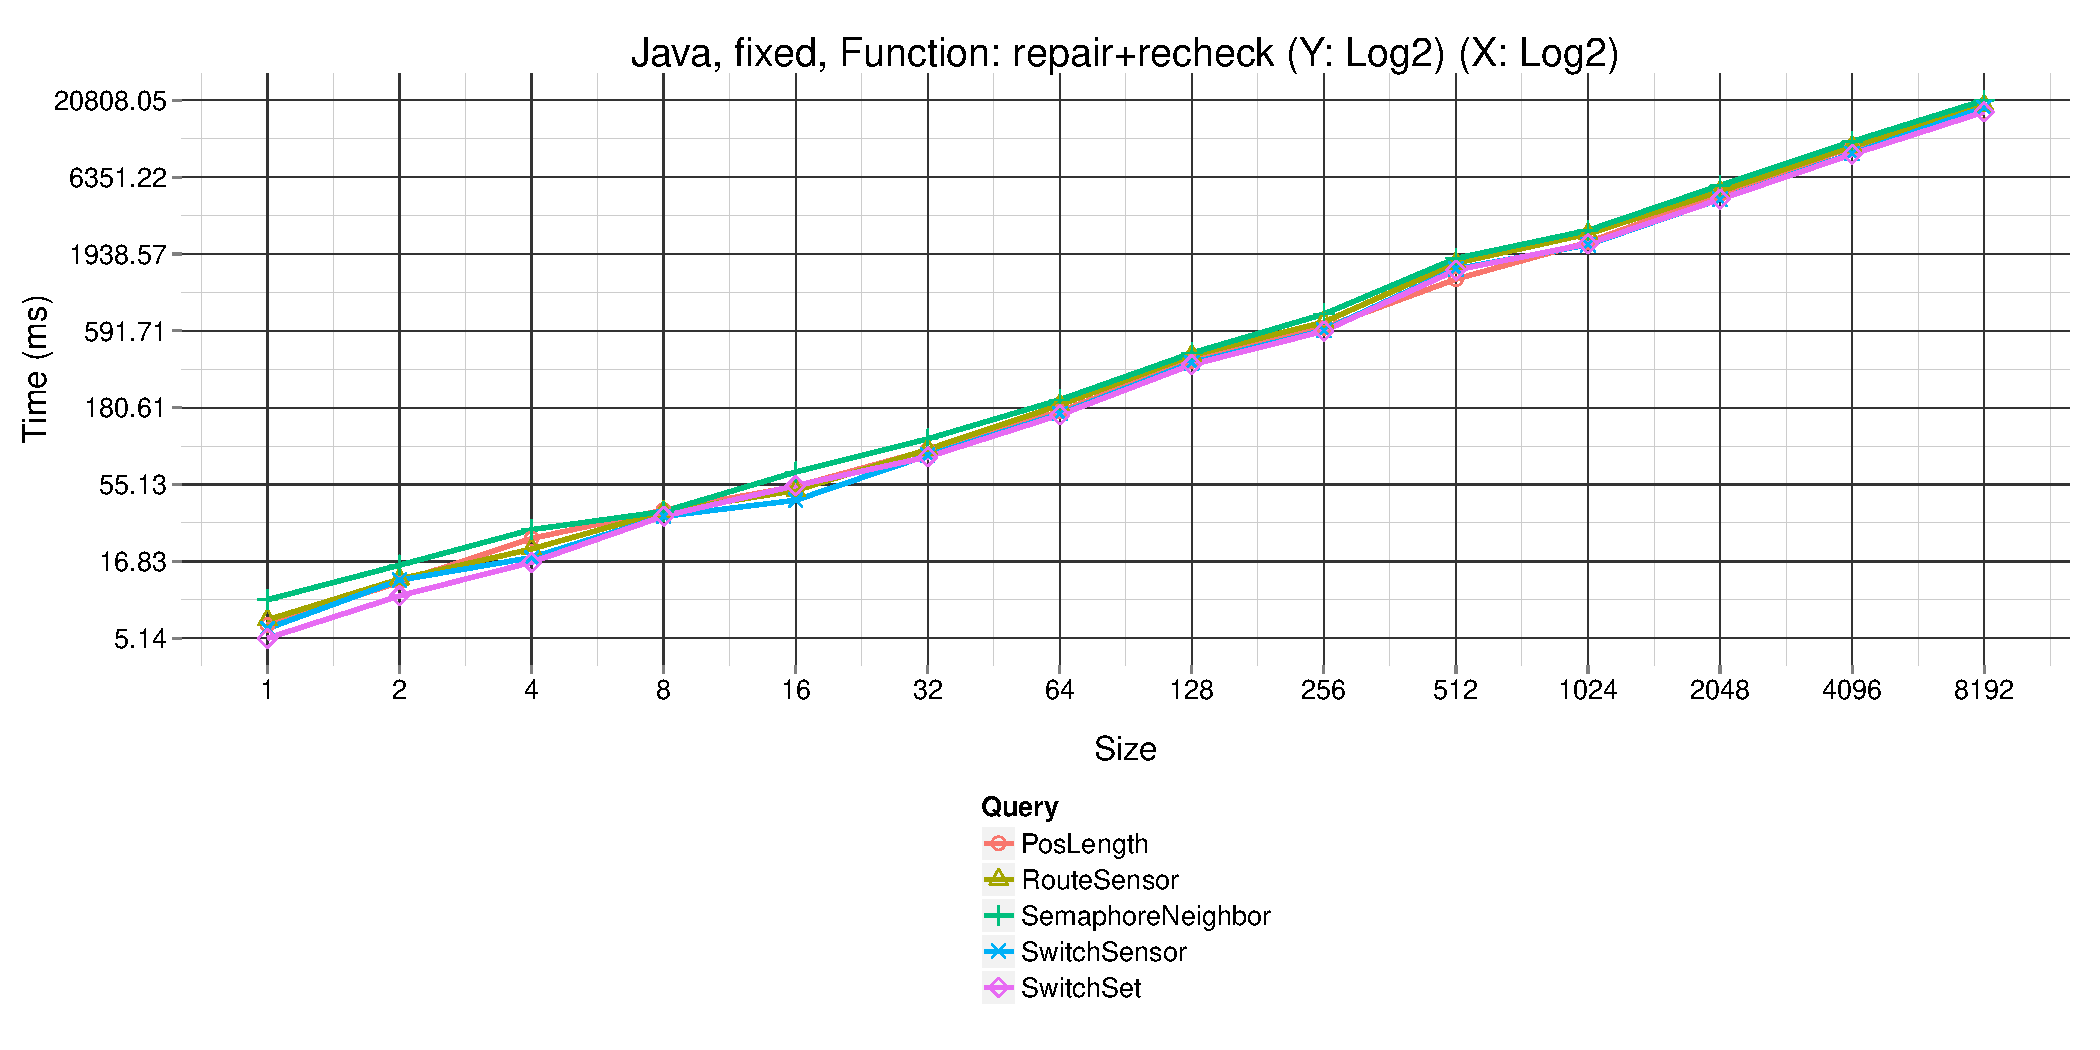
\includegraphics[width=\textwidth]{figures/fixed-Java-GroupBy-Query-time-revalidation.pdf}
  \caption{Java fixed revalidation}
  \label{fig:JavaFixedReValidationBatch}
\end{figure}

\clearpage

%!TEX root = ttc15-train-benchmark-sigma.tex

% \vspace*{-3mm}
% \enlargethispage{7mm}


% \section{Conclusion}
% \label{sec:Conclusion}


% This case study provides a good illustration for some of the capabilities of an internal DSL approach to model querying and transformation.

% Say something about Scala itself











% \vspace*{-3mm}
\paragraph{Acknowledgments}
This work is partially supported by the Datalyse project (\href{http://www.datalyse.fr/}{\Scala|www.datalyse.fr|}).
% \vspace*{-3mm}

\bibliographystyle{eptcs}
\bibliography{references.bib}	

\appendix

%!TEX root = ttc15-train-benchmark-sigma.tex

\section{Install}
\label{sec:Install}

The only requirements for running the solution is git and maven.
To reproduce the benchmark simply execute these steps in a command line:

\begin{bashcode}
$ git clone https://github.com/fikovnik/trainbenchmark-ttc
$ cd trainbenchmark-ttc
$ ./script/run.py
\end{bashcode}

\end{document}